% This tex file is available under a
% Creative Commons Attribution-Share Alike license (CC BY-SA 2.0).
% http://creativecommons.org/licenses/by-sa/2.0/
% Copyright © 2013 Rodrigo Hausen
\documentclass{beamer}
\usepackage[utf8]{inputenc}
\usepackage{lmodern}
\usepackage[T1]{fontenc}
\usepackage[portuguese,brazil]{babel}
\usepackage{url}
\usepackage{listings}
\usepackage{color}
\usepackage{textcomp}
\usepackage{pdfpages}
\usepackage{fancyvrb}
\usepackage{enumerate}
\usepackage{alltt}
\usepackage{array}
\usepackage{slashbox}
%\usepackage[pdf]{pstricks}
%\usepackage{auto-pst-pdf}
%\usepackage{icomma} % para vírgula decimal / decimal comma
\definecolor{listinggray}{gray}{0.9}
\definecolor{mediumgray}{rgb}{0.6,0.6,0.6}
\definecolor{lbcolor}{rgb}{0.9,0.9,0.9}
\lstset{
    backgroundcolor=\color{lbcolor},
    tabsize=4,
    rulecolor=,
    basicstyle=\scriptsize,
    upquote=true,
    aboveskip={1.5\baselineskip},
    columns=fixed,
    showstringspaces=false,
    extendedchars=true,
    breaklines=true,
    prebreak = \raisebox{0ex}[0ex][0ex]{\ensuremath{\hookleftarrow}},
    frame=single,
    showtabs=false,
    showspaces=false,
    showstringspaces=false,
    identifierstyle=\ttfamily,
    keywordstyle=\color[rgb]{0,0,1},
    commentstyle=\color[rgb]{0.133,0.545,0.133},
    stringstyle=\color[rgb]{0.627,0.126,0.941},
}
\definecolor{pinegreen}{RGB}{0,139,114}
\definecolor{pgr}{RGB}{0,139,114}

\definecolor{aquamarine}{RGB}{0,181,190}
\definecolor{aqm}{RGB}{0,181,190}

\definecolor{skyblue}{RGB}{100,227,251}
\definecolor{skb}{RGB}{100,227,251}

\definecolor{pnk}{RGB}{255,150,150}

\newcommand{\WD}[1]{\fbox{#1}\hspace{-0.5pt}}
\newcommand{\FWD}[1]{%
\fbox{%
\vbox to 10pt{\vfil%
\hbox to 0.8cm{\hfill#1\hfill}%
\vfil}%
}\hspace{-0.5pt}%
}

\def\A{\texttt{A}}
\def\B{\texttt{B}}
\def\C{\texttt{C}}
\def\D{\texttt{D}}
\def\E{\texttt{E}}
\def\F{\texttt{F}}

\usetheme{Boadilla}
%\usetheme{umbc2}
\usefonttheme{structuresmallcapsserif}
\usecolortheme{seahorse}

\title{Aula 9: Análise e Síntese de Circuitos Digitais Combinacionais}
\subtitle{Circuitos Digitais}
\author{Rodrigo Hausen}
\institute{CMCC -- UFABC} 
\date{25 de fevereiro de 2013}

\newcommand{\Not}[1]{\overline{#1}}
\def\And{\,}

\begin{document}

\begin{frame}
\maketitle

\vspace{-1cm}

\begin{center}
\url{http://compscinet.org/circuitos}
\end{center}

\end{frame}

%%%%%%%%%%%%%%%%%%%%%%%%%%%%%%%%%%%%%%%%%%%%%%%%%

\begin{frame}
\frametitle{Portas lógicas}

\begin{itemize}
\item circuitos que efetuam operações básicas da álgebra booleana
\end{itemize}

\uncover<2->{
\begin{minipage}{0.4\textwidth}
\begin{center}
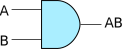
\includegraphics{images/and_gate} \\
Porta \textbf{and}
\vspace*{12pt}
\end{center}
\end{minipage}
}
\hspace*{4ex}
\begin{minipage}{0.4\textwidth}
\begin{center}

\includegraphics{images/not_gate}\\
Porta \textbf{not}
\vspace*{12pt}
\end{center}
\end{minipage}

\uncover<3->{
\begin{minipage}{0.4\textwidth}
\begin{center}
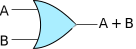
\includegraphics{images/or_gate} \\
Porta \textbf{or}
\vspace*{12pt}
\end{center}
\end{minipage}
}

\uncover<4->{
\begin{minipage}{0.4\textwidth}
\begin{center}
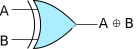
\includegraphics{images/xor_gate} \\
Porta \textbf{xor}
\vspace*{12pt}
\end{center}
\end{minipage}
}

\end{frame}

%%%%%%%%%%%%%%%%%%%%%%%%%%%%%%%%%%%%%%%%%%%%%%%%%

\begin{frame}
\frametitle{Portas lógicas com saída invertida}

\begin{itemize}
\item também existem as seguintes portas com saída invertida (negada)
\end{itemize}

\uncover<2->{
\begin{minipage}[c]{0.4\textwidth}
\begin{center}
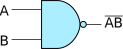
\includegraphics{images/nand_gate} \\
Porta \textbf{nand}
\vspace*{12pt}
\end{center}
\end{minipage}
}
\uncover<5->{
\hspace{2ex}
{\Huge $\equiv$}
\hspace{2ex}
\begin{minipage}[c]{0.4\textwidth}

\includegraphics{images/nand_circ}
\end{minipage}
}

\uncover<3->{
\begin{minipage}{0.4\textwidth}
\begin{center}
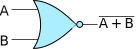
\includegraphics{images/nor_gate} \\
Porta \textbf{nor}
\vspace*{12pt}
\end{center}
\end{minipage}
}
\uncover<6->{
\hspace{2ex}
{\Huge $\equiv$}
\hspace{2ex}
\begin{minipage}[c]{0.4\textwidth}
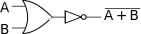
\includegraphics{images/nor_circ}
\end{minipage}
}


\uncover<4->{
\begin{minipage}{0.4\textwidth}
\begin{center}
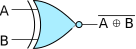
\includegraphics{images/xnor_gate} \\
Porta \textbf{xnor}
\vspace*{12pt}
\end{center}
\end{minipage}
}
\uncover<7->{
\hspace{2ex}
{\Huge $\equiv$}
\hspace{2ex}
\begin{minipage}[c]{0.4\textwidth}
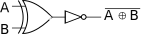
\includegraphics{images/xnor_circ}
\end{minipage}
}

\end{frame}

%%%%%%%%%%%%%%%%%%%%%%%%%%%%%%%%%%%%%%%%%%%%%%%%%

\begin{frame}
\frametitle{Observações sobre portas lógicas}

\begin{itemize}
\item Quaisquer portas lógicas podem ser construídas usando-se apenas as portas básicas \textbf{not}, \textbf{and} com duas entradas e \textbf{or} com duas entradas.
\pause
\item Exemplo A: \textbf{and} com $5$ entradas

\hspace{3ex}
\begin{tabular}{m{20ex}m{6ex}m{24ex}}

\includegraphics{images/and5_gate} \pause & {\Huge =} & 
\includegraphics{images/and5_circ}
\\[12pt]
\end{tabular}
\pause
\item Exemplo B: \textbf{xor} com $2$ entradas (na lousa)
\end{itemize}


\end{frame}

%%%%%%%%%%%%%%%%%%%%%%%%%%%%%%%%%%%%%%%%%%%%%%%%%

\begin{frame}
\frametitle{Observações sobre portas lógicas}

{\small
\begin{itemize}

\item Geralmente, usamos portas lógicas encontradas em circuitos integrados. \pause Por exemplo: 7408 ($4$ portas \textbf{and} com $2$ entradas)
\end{itemize}

\hfill 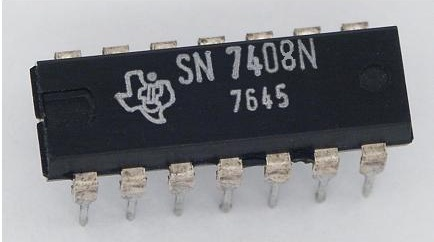
\includegraphics[width=0.4\textwidth]{images/7408foto} \hfill 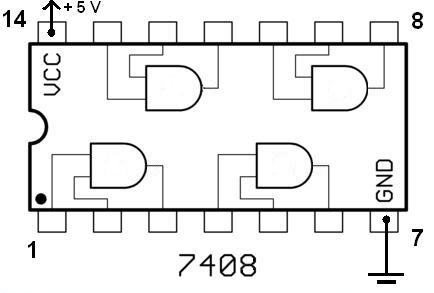
\includegraphics[width=0.4\textwidth]{images/7408circ} \hfill \phantom{.}\\ 
{\hfill \color{gray} \tiny Fonte da imagem: \url{http://en.wikipedia.org/wiki/File:7400.jpg} (imagem alterada)}

\pause

\begin{itemize}
\item Encontram-se circuitos integrados para o inversor (7404 / CD4049) e para as portas de $2$ entradas: \textbf{and} (7408 / CD4081), \textbf{or} (7432 / CD4071), \textbf{xor} (7486), \textbf{nand} (7400 / CD4012) e \textbf{nor} (7402 / CD4001) e \textbf{xnor} (CD4077).
\pause
\begin{itemize}
\item 74xx -- tradicionalmente de tecnologia TTL (74LSxx)
\item CD40xx -- tecnologia CMOS
\end{itemize}

\pause

\item Também encontram-se portas lógicas com até $8$ entradas
\end{itemize}
}

\end{frame}

%%%%%%%%%%%%%%%%%%%%%%%%%%%%%%%%%%%%%%%%%%%%%%%%%

\begin{frame}
\frametitle{Análise de circuitos digitais}

\begin{itemize}
\item \textbf{Exemplo 1}: Dado o circuito abaixo, encontre uma expressão lógica para $E$ em função de $A$, $B$, $C$ e $D$.\\[6pt]

\only<1>{
\begin{picture}(224,170)(0,0)
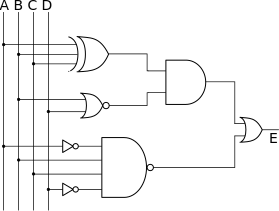
\includegraphics{images/exemplo3}
\end{picture}
}

\only<2>{
\begin{picture}(224,170)(0,0)
\put(89,130){\footnotesize $A \oplus B \oplus C$}
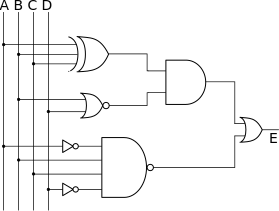
\includegraphics{images/exemplo3}
\end{picture}
}

\only<3>{
\begin{picture}(224,170)(0,0)
\put(89,130){\footnotesize $A \oplus B \oplus C$}
\put(89,88){\footnotesize $\overline{B + D}$}
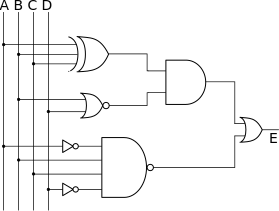
\includegraphics{images/exemplo3}
\end{picture}
}

\only<4>{
\begin{picture}(224,170)(0,0)
\put(89,130){\footnotesize $A \oplus B \oplus C$}
\put(89,88){\footnotesize $\overline{B + D}$}
\put(69,55){\footnotesize $\overline{A}$}%
\put(69,44){\footnotesize $B$}%
\put(69,32){\footnotesize $C$}%
\put(69,20){\footnotesize $\overline{D}$}%
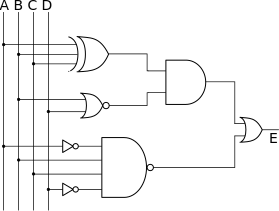
\includegraphics{images/exemplo3}
\end{picture}
}

\only<5>{
\begin{picture}(224,170)(0,0)
\put(89,130){\footnotesize $A \oplus B \oplus C$}
\put(89,88){\footnotesize $\overline{B + D}$}
\put(69,55){\footnotesize $\overline{A}$}%
\put(69,44){\footnotesize $B$}%
\put(69,32){\footnotesize $C$}%
\put(69,20){\footnotesize $\overline{D}$}%
\put(128,39){\footnotesize $\overline{\overline{A}BC\overline{D}}$}
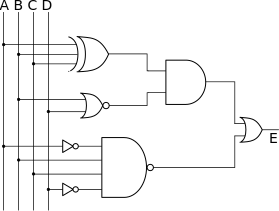
\includegraphics{images/exemplo3}
\end{picture}
}

\only<6>{
\begin{picture}(224,170)(0,0)
\put(89,130){\footnotesize $A \oplus B \oplus C$}
\put(89,88){\footnotesize $\overline{B + D}$}
\put(69,55){\footnotesize $\overline{A}$}%
\put(69,44){\footnotesize $B$}%
\put(69,32){\footnotesize $C$}%
\put(69,20){\footnotesize $\overline{D}$}%
\put(128,39){\footnotesize $\overline{\overline{A}BC\overline{D}}$}
\put(170,108){\footnotesize $(A \oplus B \oplus C) \cdot \overline{B + D}$}
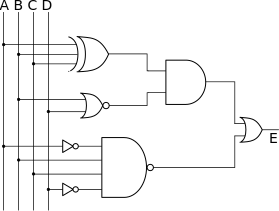
\includegraphics{images/exemplo3}
\end{picture}
}

\only<7->{
\begin{picture}(224,170)(0,0)
\put(89,130){\footnotesize $A \oplus B \oplus C$}
\put(89,88){\footnotesize $\overline{B + D}$}
\put(69,55){\footnotesize $\overline{A}$}%
\put(69,44){\footnotesize $B$}%
\put(69,32){\footnotesize $C$}%
\put(69,20){\footnotesize $\overline{D}$}%
\put(128,39){\footnotesize $\overline{\overline{A}BC\overline{D}}$}
\put(170,108){\footnotesize $(A \oplus B \oplus C) \cdot \overline{B + D}$}
\put(214,85){\footnotesize $\left( (A \oplus B \oplus C) \cdot \overline{B + D} \right) + $}
\put(214,69){\footnotesize $+ \overline{\overline{A}BC\overline{D}}$}
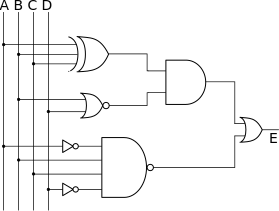
\includegraphics{images/exemplo3}
\end{picture}
}

\uncover<8>{Resp.: $E = \left( (A \oplus B \oplus C) \cdot \overline{B + D} \right) + \overline{\overline{A}BC\overline{D}}$}

\end{itemize}

\end{frame}

%%%%%%%%%%%%%%%%%%%%%%%%%%%%%%%%%%%%%%%%%%%%%%%%%

\begin{frame}
\frametitle{Análise de circuitos digitais}

\begin{itemize}
\item \textbf{Exemplo 2}: Encontre uma expressão lógica para cada saída. 
\end{itemize}

\begin{center}
\only<1-2>{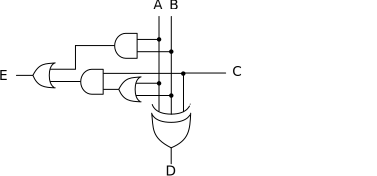
\includegraphics{images/analise2}}%
\only<3>{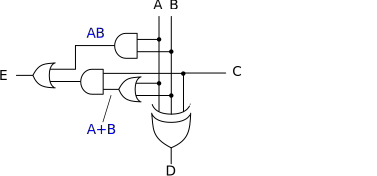
\includegraphics{images/analise2_2}}%
\only<4->{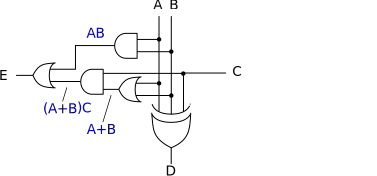
\includegraphics{images/analise2_3}}%
\end{center}

\uncover<2->{Resposta: $D = A \oplus B \oplus C$}\\
\uncover<5->{\hspace{10ex}$E = AB + (A+B)C$}
\end{frame}

%%%%%%%%%%%%%%%%%%%%%%%%%%%%%%%%%%%%%%%%%%%%%%%%%

\begin{frame}
\frametitle{Análise de circuitos digitais}

\begin{itemize}
\item \textbf{Tenha sempre em mente:}\\ para obter a expressão lógica nas saídas
de um circuito digital, vá ``caminhando'' das entradas em direção às
saídas, escrevendo no saída de cada porta lógica a expressão equivalente.
\end{itemize}

\end{frame}

%%%%%%%%%%%%%%%%%%%%%%%%%%%%%%%%%%%%%%%%%%%%%%%%%

\begin{frame}
\frametitle{Análise via formas de onda}

\begin{itemize}
\item Em um determinado instante, um sinal digital está em \emph{apenas um}
dos seguintes estados:
\begin{itemize}
\item nível \textbf{baixo} = 0; ou
\item nível \textbf{alto} = 1
\end{itemize}
\pause
\item Porém, o estado de um sinal digital \textbf{pode variar com o tempo}.
Demonstramos essa variação por meio de \textbf{diagramas de forma de onda}:
\end{itemize}
\begin{center}
\only<1-2>{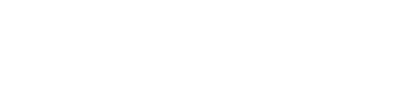
\includegraphics{images/waveform1_empty}}%
\only<3>{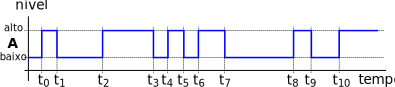
\includegraphics{images/waveform1_0}}%
\only<4->{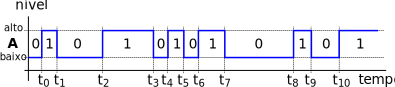
\includegraphics{images/waveform1}}
\end{center}

\end{frame}

%%%%%%%%%%%%%%%%%%%%%%%%%%%%%%%%%%%%%%%%%%%%%%%%%

\begin{frame}
\frametitle{Análise via formas de onda}

\begin{itemize}
\item \textbf{Exemplo 3:} Esboce o diagrama de forma de onda para a saída
$B$, considerando a forma de onda de entrada.
\end{itemize}
\begin{center}

\includegraphics{images/waveform2_circ}\\[12pt]
\only<1>{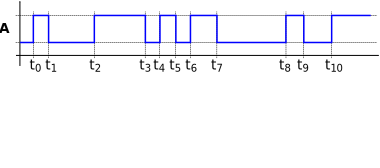
\includegraphics{images/waveform2_1}}%
\only<2>{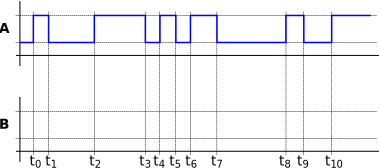
\includegraphics{images/waveform2_2}}%
\only<3>{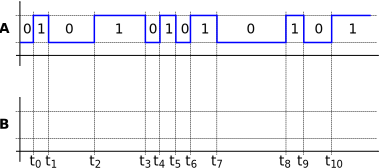
\includegraphics{images/waveform2_3}}%
\only<4>{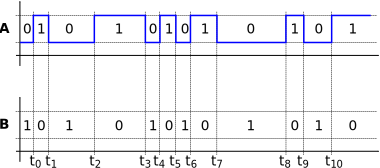
\includegraphics{images/waveform2_4}}%
\only<5>{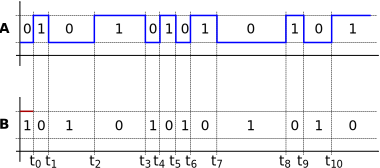
\includegraphics{images/waveform2_5}}%
\only<6>{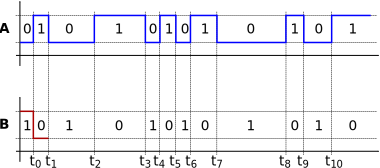
\includegraphics{images/waveform2_6}}%
\only<7>{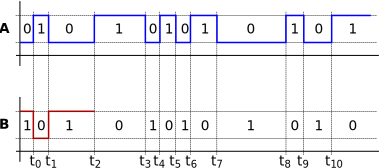
\includegraphics{images/waveform2_7}}%
\only<8>{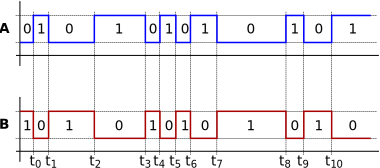
\includegraphics{images/waveform2_8}}%
\only<9>{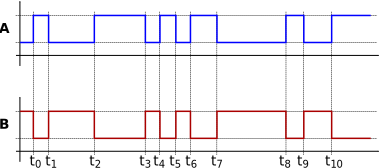
\includegraphics{images/waveform2_9}}%
\end{center}
\end{frame}

%%%%%%%%%%%%%%%%%%%%%%%%%%%%%%%%%%%%%%%%%%%%%%%%%

\begin{frame}
\frametitle{Análise via formas de onda}

\begin{itemize}
\item \textbf{Exemplo 4:} Esboce o diagrama de forma de onda para a saída
$C$, considerando as formas de onda das entradas $A,B$.
\end{itemize}
\begin{center}

\includegraphics{images/waveform3_circ}\\[6pt]
\only<1>{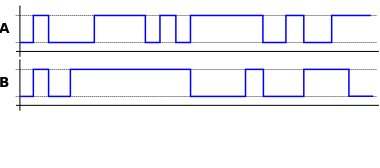
\includegraphics{images/waveform3_1}}%
\only<2>{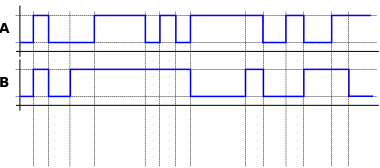
\includegraphics{images/waveform3_2}}%
\only<3>{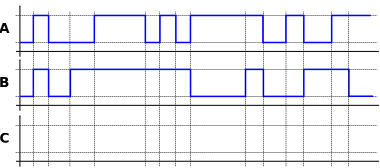
\includegraphics{images/waveform3_3}}%
\only<4>{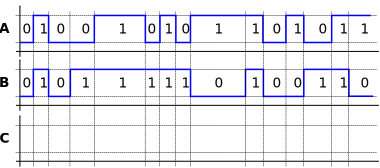
\includegraphics{images/waveform3_4}}%
\only<5>{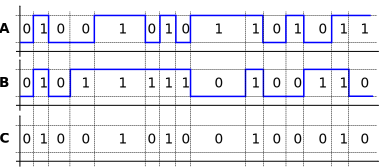
\includegraphics{images/waveform3_5}}%
\only<6>{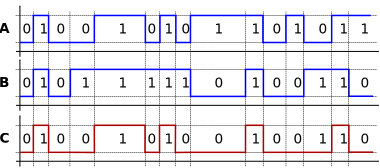
\includegraphics{images/waveform3_6}}%
\only<7>{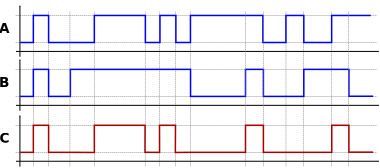
\includegraphics{images/waveform3_7}}%
\end{center}
\end{frame}

%%%%%%%%%%%%%%%%%%%%%%%%%%%%%%%%%%%%%%%%%%%%%%%%%

\begin{frame}
\frametitle{Análise via formas de onda: observações}

\begin{itemize}
\item O eixo horizontal será sempre o tempo, o eixo vertical será o nível de cada sinal.
\pause
\item Geralmente, as entradas e saídas são colocadas no mesmo gráfico. Ex:\\
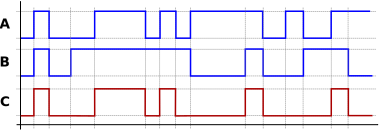
\includegraphics{images/waveform4}
\pause
\item Neste curso, assumiremos sempre circuitos ideais: forma de onda
ideal (sem distorções), transições instantâneas entre estados, nenhum
atraso entre entradas e saídas.
\begin{itemize}
\item em outras palavras: $V_{high}$ e $V_{low}$ sempre constantes distintas,\\
slew rate = ``$\infty$'', delay = 0 para qualquer porta lógica ou fio.
\end{itemize}
\end{itemize}

\end{frame}

%%%%%%%%%%%%%%%%%%%%%%%%%%%%%%%%%%%%%%%%%%%%%%%%%

\begin{frame}
\frametitle{Análise via formas de onda}

\begin{itemize}
\item \textbf{Exemplo 5:} Esboce o diagrama de forma de onda das saídas,
considerando o diagrama de forma de onda das entradas.
\end{itemize}
\begin{center}
\begin{minipage}{0.5\textwidth}
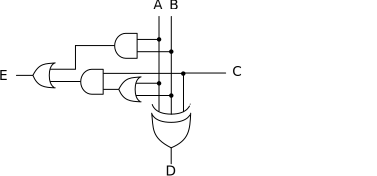
\includegraphics[scale=0.7]{images/analise2}
\end{minipage}
\begin{minipage}{0.4\textwidth}
\uncover<2->{
\textbf{Primeiro passo:} obter uma expressão para cada saída.\\
Já fizemos antes:\\
$D = A \oplus B \oplus C$\\
$E = AB + (A+B)C$
}
\end{minipage}\\
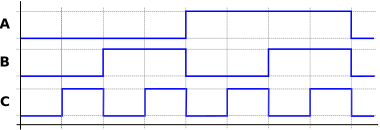
\includegraphics[scale=0.7]{images/waveform5}
\end{center}

\end{frame}

%%%%%%%%%%%%%%%%%%%%%%%%%%%%%%%%%%%%%%%%%%%%%%%%%

\begin{frame}
\frametitle{Análise via formas de onda}

\begin{itemize}
\item \textbf{Segundo passo (opcional):} obter tabela verdade para cada
saída.
\pause
\begin{itemize}
\item $D = A \oplus B \oplus C$ será 1 apenas se número ímpar de entradas é 1
\pause
\item $E = AB + (A+B)C$\\[6pt]
\pause
\begin{tabular}{ccc||c}
A & B & C & E \\
\hline
0 & 0 & 0 & 0 \\
0 & 0 & 1 & 0 \\
0 & 1 & 0 & 0 \\
0 & 1 & 1 & 1 \\
1 & 0 & 0 & 0 \\
1 & 0 & 1 & 1 \\
1 & 1 & 0 & 1 \\
1 & 1 & 1 & 1
\end{tabular}
\end{itemize}
\pause
\item \textbf{Terceiro passo: } esboçar os diagramas de formas de onda das saídas, com o auxílio das tabelas verdade obtidas no passo anterior, se necessário.
\end{itemize}

\end{frame}

%%%%%%%%%%%%%%%%%%%%%%%%%%%%%%%%%%%%%%%%%%%%%%%%%

\begin{frame}
\frametitle{Análise via formas de onda}

\begin{itemize}
\item \textbf{Terceiro passo: } esboçar os diagramas de formas de onda das saídas, com o auxílio das tabelas verdade obtidas no passo anterior, se necessário.
\end{itemize}
\begin{center}
\only<1>{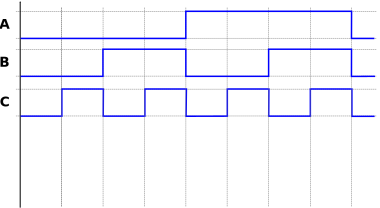
\includegraphics{images/waveform5_1}}%
\only<2>{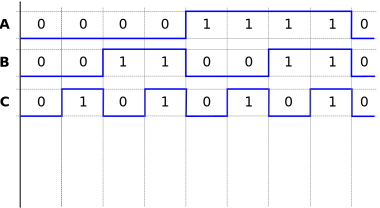
\includegraphics{images/waveform5_2}}%
\only<3>{\includegraphics{images/waveform5_3}}%
\only<4>{\includegraphics{images/waveform5_4}}%
\only<5>{\includegraphics{images/waveform5_5}}%
\only<6>{\includegraphics{images/waveform5_6}}%
\only<7>{\includegraphics{images/waveform5_7}}%
\only<8>{\includegraphics{images/waveform5_8}}%
\end{center}

\end{frame}


%%%%%%%%%%%%%%%%%%%%%%%%%%%%%%%%%%%%%%%%%%%%%%%%%

\begin{frame}
\frametitle{Síntese de circuitos digitais}

\begin{itemize}
\item \textbf{Exemplo 6}: Elabore um circuito com portas lógicas \textbf{not}, \textbf{and} e \textbf{or} cuja saída corresponda à expressão $A \oplus B$ ($A$ \textbf{xor} $B$).\\[6pt]

\pause

Sabemos que $A \oplus B = \overline{A}B + A\overline{B}$\\[6pt]
\end{itemize}

\pause

\begin{center}
\includegraphics[scale=0.8]{images/exemplo1}
\end{center}

\pause

\begin{itemize}
\item geralmente não representamos, em um circuito digital, onde está a fonte de tensão/bateria
\pause
\item recomenda-se colocar as entradas ``na vertical'' e desenvolver as saídas ``na horizontal, para a direita''

\end{itemize}

\end{frame}

%%%%%%%%%%%%%%%%%%%%%%%%%%%%%%%%%%%%%%%%%%%%%%%%%

\begin{frame}
\frametitle{Síntese de circuitos digitais}

\def\Zero{\raisebox{0pt}{\color{structure.fg!70!white}0}}

\begin{itemize}
\item \textbf{Exemplo 7}: Elabore um circuito com portas lógicas \textbf{not}, \textbf{and} e \textbf{or} cuja saída corresponda à função lógica $C(V,F,U,N)$, onde\\[12pt]
\begin{tabular}{c@{ }c@{ }c@{ }c||c@{ }l}
 $V$ & $F$ & $U$ & $N$ & $C$ \\
\cline{1-5}
  0  &  0  &  0  &  0  &  \Zero  \\
  0  &  0  &  0  &  1  &  \Zero  \\
  0  &  0  &  1  &  0  &  \Zero  \\
  0  &  0  &  1  &  1  &  1  \\
  0  &  1  &  0  &  0  &  \Zero  \\
  0  &  1  &  0  &  1  &  1  \\
  0  &  1  &  1  &  0  &  1  \\
  0  &  1  &  1  &  1  &  1  \\
\end{tabular}
\hspace{4ex}
\begin{tabular}{c@{ }c@{ }c@{ }c||cl}
 $V$ & $F$ & $U$ & $N$ & $C$ \\
\cline{1-5}
  1  &  0  &  0  &  0  &  \Zero  \\
  1  &  0  &  0  &  1  &  1  \\
  1  &  0  &  1  &  0  &  1  \\
  1  &  0  &  1  &  1  &  \Zero  \\
  1  &  1  &  0  &  0  &  \Zero  \\
  1  &  1  &  0  &  1  &  \Zero  \\
  1  &  1  &  1  &  0  &  1  \\
  1  &  1  &  1  &  1  &  1  \\
\end{tabular}
\end{itemize}

\pause

\begin{itemize}
\item \textbf{Primeiro passo: } obtenha e simplifique a expressão lógica para as saídas.
\end{itemize}

\end{frame}

%%%%%%%%%%%%%%%%%%%%%%%%%%%%%%%%%%%%%%%%%%%%%%%%%

\begin{frame}
\frametitle{Síntese de circuitos digitais}

\begin{itemize}
\item \textbf{Primeiro passo: } obtenha e simplifique a expressão lógica para as saídas.\\[6pt]
Mapa de Karnaugh para a tabela verdade dada:
\begin{center}
\only<01>{\includegraphics{images/kmap01}}%
\only<02->{\includegraphics{images/kmap01_15}}%
\end{center}

\pause\pause

$C = V \And \Not{F} \And \Not{U} \And N + {\color{gray} V \And U \And \Not{N}} + {\color{pinegreen} \Not{V} \And U \And N} + {\color{blue} \Not{V} \And F \And N} + {\color{red} F \And U }$ 

\end{itemize}

\end{frame}

%%%%%%%%%%%%%%%%%%%%%%%%%%%%%%%%%%%%%%%%%%%%%%%%%

\begin{frame}
\frametitle{Síntese de circuitos digitais}

\begin{itemize}
\item \textbf{Segundo passo: } desenhar o diagrama do circuito.
\end{itemize}

\begin{center}
\only<1>{\includegraphics[height=35ex]{images/exemplo2_empty}}%
\only<2-3>{\includegraphics[height=35ex]{images/exemplo2}}%
\only<4>{\includegraphics[height=35ex]{images/exemplo2_econ}}%
\end{center}

\vspace{-12pt}

\only<1-2>{\phantom{note que estamos sendo pouco econômicos com as portas not}}%
\only<3>{note que estamos sendo pouco econômicos com as portas not}%
\only<4>{economizamos uma porta not}%

\end{frame}

%%%%%%%%%%%%%%%%%%%%%%%%%%%%%%%%%%%%%%%%%%%%%%%%%

\begin{frame}
\frametitle{Síntese de circuitos digitais}

\begin{itemize}
\item \textbf{Terceiro passo: } analizar o circuito e verificar as saídas
\end{itemize}

\begin{center}
\only<1>{\includegraphics[height=40ex]{images/exemplo2_econ0}}%
\only<2>{\includegraphics[height=40ex]{images/exemplo2_econ1}}%
\only<3>{\includegraphics[height=40ex]{images/exemplo2_econ2}}%
\only<4>{\includegraphics[height=40ex]{images/exemplo2_econ}}%
\end{center}

\end{frame}

%%%%%%%%%%%%%%%%%%%%%%%%%%%%%%%%%%%%%%%%%%%%%%%%%

\begin{frame}
\frametitle{Síntese de circuitos digitais}

\begin{itemize}
\item \textbf{Quarto passo: } montar o circuito e fazer a sua tabela verdade.

\pause

\item A partir de agora, usaremos o simulador de circuitos Logisim:\\
      \url{http://ozark.hendrix.edu/~burch/logisim/pt/index.html}

\pause

\item Na prática, além de simular, você irá montar o seu circuito em um protoboard ou placa padrão:\\
\includegraphics[width=20ex]{images/breadboard}\hspace{5ex}
{\color{gray}\tiny\url{http://en.wikipedia.org/wiki/File:Breadboard.JPG}}

\end{itemize}

\end{frame}

%%%%%%%%%%%%%%%%%%%%%%%%%%%%%%%%%%%%%%%%%%%%%%%%%

\begin{frame}
\frametitle{Síntese de circuitos digitais}

\begin{itemize}
\item \textbf{Erros comuns: } (1) esquecer de fazer a soma dos produtos\\
(ou seja, omitir a porta or)
\end{itemize}

\begin{center}
\only<1>{\includegraphics[height=35ex]{images/exemplo2_err1}}%
\only<2>{\includegraphics[height=35ex]{images/exemplo2_err1_2}}%
\end{center}

\end{frame}

%%%%%%%%%%%%%%%%%%%%%%%%%%%%%%%%%%%%%%%%%%%%%%%%%

\begin{frame}
\frametitle{Síntese de circuitos digitais}

\begin{itemize}
\item \textbf{Erros comuns: } (2) juntar as saídas sem colocar porta or\\
(queima as portas lógicas, ou resultado indeterminado!)
\end{itemize}

\begin{center}
\only<1>{\includegraphics[height=35ex]{images/exemplo2_err2}}%
\only<2>{\includegraphics[height=35ex]{images/exemplo2_err2_2}}%
\end{center}

\end{frame}

%%%%%%%%%%%%%%%%%%%%%%%%%%%%%%%%%%%%%%%%%%%%%%%%%

\begin{frame}
\frametitle{Síntese de circuitos digitais}

\begin{itemize}
\item \textbf{Correto: } verifique sempre o seu circuito.
\end{itemize}

\begin{center}
\includegraphics[height=35ex]{images/exemplo2_econ}
\end{center}

\end{frame}

%%%%%%%%%%%%%%%%%%%%%%%%%%%%%%%%%%%%%%%%%%%%%%%%%

\begin{frame}
\frametitle{Síntese de circuitos digitais}

\textbf{Resumo: } Os quatro passos para um circuito digital feliz.

\begin{itemize}

\item \textbf{Primeiro passo: } obtenha e simplifique a expressão lógica para cada saída.

\pause

\item \textbf{Segundo passo: } desenhe o diagrama do circuito.

\pause

\begin{itemize}
\item cuidado com os erros comuns: esquecer portas lógicas, juntar saídas sem
usar porta lógica, etc.
\end{itemize}

\pause

\item \textbf{Terceiro passo: } analize o circuito e verifique as saídas.

\pause

\begin{itemize}
\item vá ``caminhando'' das entradas em direção às
saídas, escrevendo na saída de cada porta lógica a expressão equivalente.
\end{itemize}

\pause

\item \textbf{Quarto passo: } monte o circuito, faça a sua tabela verdade e
verifique se ela coincide com as tabelas verdade das expressões obtidas
no primeiro passo.

\pause

\begin{itemize}
\item primeiro simule, depois monte o circuito em uma placa padrão
\end{itemize}

\end{itemize}

\end{frame}

%%%%%%%%%%%%%%%%%%%%%%%%%%%%%%%%%%%%%%%%%%%%%%%%%

\begin{frame}
\frametitle{Para casa:}

\begin{itemize}
\item Determine a expressão lógica mais simples para a saída de cada um dos
circuitos abaixo (os circuitos usam apenas portas \textbf{nand})
\end{itemize}
\begin{center}
\begin{minipage}{0.2\textwidth}
\includegraphics[scale=0.9]{images/nand_univ1}\\
Circuito 1
\end{minipage}
\hspace{8ex}
\begin{minipage}{0.4\textwidth}
\includegraphics[scale=0.9]{images/nand_univ2}\\
Circuito 2
\end{minipage}

\vspace{12pt}

\includegraphics[scale=0.9]{images/nand_univ3}\\
Circuito 3
\end{center}
\begin{itemize}
\item O que você pode concluir deste exercício?
\end{itemize}
 
\end{frame}

%%%%%%%%%%%%%%%%%%%%%%%%%%%%%%%%%%%%%%%%%%%%%%%%%

\begin{frame}
\frametitle{Para casa:}

\begin{itemize}
\item Se você ainda não fez, faça \textbf{imediatamente} a leitura
recomendada e os exercícios da aula passada.
Refaça os exercícios 13 a 16 da aula passada usando o Logisim.
\item Ler seções 1-2 e 1-3. Ler 1-5 apenas como cultura geral.
\item Exercícios do cap. 1: autoteste 3 a 8, problemas 3, 4, 10, 12, 13, 14.
\item Ler seções 3-1 a 3-6.
\item Exercícios do cap. 3: autoteste 1 a 7, problemas 1 a 22.
\item Ler seção 4-4.
\item Exercícios do cap. 4: problemas 12 a 15, 20, 34 e 44 (nestes dois
últimos, minimizar a expressão e fazer o diagrama do circuito digital).
\item Ler seções 5-1, 5-2 e 5-5.
\item Exercícios do cap. 5: autoteste 1 a 6, problemas 1 a 17, 26 a 29.
\end{itemize}

\end{frame}

\end{document}


%%%%%%%%%%%%%%%%%%%%%%%%%%%%%%%%%%%%%%%%%%%%%%%%%

\begin{frame}
\frametitle{Blocos somadores digitais}

\begin{itemize}
\item \textbf{Exemplo 4}: Elabore um circuito digital com $2$ entradas, $a_0$ e $b_0$, e $2$ saídas, $s_1$ e $s_0$ de tal forma que $(s_1 s_0)_2$ represente a soma aritmética $a_0 + b_0$.
\vspace{-12pt}
\begin{center}
\begin{tabular}{cc@{}c@{\,}c}
  && & $a_0$ \\
+ && & $b_0$ \\
\cline{2-4}
  && $s_1$ & $s_0$
\end{tabular}
\end{center}

\pause

\item \textbf{Primeiro passo}: construir as tabelas verdade para $s_1$ e $s_0$.

\pause

\begin{center}
\begin{tabular}{cc||c}
$a_0$ & $b_0$ & $s_0$ \\
\hline
  0   &   0   &   0   \\
  0   &   1   &   1   \\
  1   &   0   &   1   \\
  1   &   1   &   0
\end{tabular}
\hspace{6ex}
\begin{tabular}{cc||c}
$a_0$ & $b_0$ & $s_1$ \\
\hline
  0   &   0   &   0   \\
  0   &   1   &   0   \\
  1   &   0   &   0   \\
  1   &   1   &   1
\end{tabular}
\end{center}

\pause

\item \textbf{Segundo passo}: simplificar as tabelas verdade e obter uma expressão lógica para cada saída. Normalmente, usam-se mapas de Karnaugh e regras da álgebra booleana.\\
\pause
Neste caso, é muito simples: $s_0 = a_0 \oplus b_0$ \; e \; $s_1 = a_0 b_0$

\end{itemize}


\end{frame}

%%%%%%%%%%%%%%%%%%%%%%%%%%%%%%%%%%%%%%%%%%%%%%%%%

\begin{frame}
\frametitle{Blocos somadores digitais}

\begin{itemize}
\item \textbf{Exemplo 4}: Elabore um circuito digital com $2$ entradas, $a_0$ e $b_0$, e $2$ saídas, $s_1$ e $s_0$ de tal forma que $(s_1 s_0)_2$ represente a soma aritmética $a_0 + b_0$.

\item \textbf{Terceiro passo}: construir o circuito a partir da(s) expressão(ões) lógica(s) da(s) saída(s).\\
$s_0 = a_0 \oplus b_0$ \; e \; $s_1 = a_0 b_0$ (note que há um \textbf{and} implícito)\\[6pt]

\begin{center}
\only<1>{\includegraphics{images/exemplo4_0}}%
\only<2>{\includegraphics{images/exemplo4_1}}%
\only<3>{\includegraphics{images/exemplo4_2}}%
\only<4>{\includegraphics{images/exemplo4_3}}%
\only<5>{\includegraphics{images/exemplo4}}
\end{center}

\end{itemize}
\end{frame}


%%%%%%%%%%%%%%%%%%%%%%%%%%%%%%%%%%%%%%%%%%%%%%%%%

\newcommand{\INP}[1]{\fcolorbox{white}{pnk}{#1}}
\newcommand{\OUT}[1]{\fcolorbox{white}{skb}{#1}}

\begin{frame}
\frametitle{Blocos somadores digitais}

\begin{itemize}
\item \textbf{Exemplo 5}: Elabore um circuito digital com $3$ entradas, $a_i$, $b_i$, $c_{i-1}$ e $2$ saídas, $s_i$ e $c_i$ de tal forma que $s_i$ represente a soma aritmética $a_i + b_i + c_{i-1}$ e $c_i$ represente o vai-um (carry) da operação.

\end{itemize}

\begin{center}
\begin{tabular}{rc@{}c@{\,}c@{\,}c@{\,}c@{\,}c@{\,}c}
vai-uns $\rightarrow$
 & & $c_{i+1}$ & \OUT{$c_{i}$} & \INP{$c_{i-1}$}           & \ldots & $c_0$ &       \\
 & & \ldots    & $a_{i+1}$     & \INP{$a_{i\phantom{-1}}$} & \ldots & $a_1$ & $a_0$ \\
+& & \ldots    & $b_{i+1}$     & \INP{$b_{i\phantom{-1}}$} & \ldots & $b_1$ & $b_0$ \\
\cline{2-8}
 & & \ldots    & $s_{i+1}$     & \OUT{$s_{i\phantom{-1}}$} & \ldots & $s_1$ & $s_0$
\end{tabular}
\end{center}

\end{frame}

%%%%%%%%%%%%%%%%%%%%%%%%%%%%%%%%%%%%%%%%%%%%%%%%%
\begin{frame}
\frametitle{Blocos somadores digitais}

\begin{itemize}
\item \textbf{Primeiro passo}: tabelas verdade.
\end{itemize}

\begin{center}
\begin{tabular}{rc@{}c@{\,}c@{\,}c@{\,}c@{\,}c@{\,}c}
vai-uns $\rightarrow$
 & & $c_{i+1}$ & \OUT{$c_{i}$} & \INP{$c_{i-1}$}           & \ldots & $c_0$ &       \\
 & & \ldots    & $a_{i+1}$     & \INP{$a_{i\phantom{-1}}$} & \ldots & $a_1$ & $a_0$ \\
+& & \ldots    & $b_{i+1}$     & \INP{$b_{i\phantom{-1}}$} & \ldots & $b_1$ & $b_0$ \\
\cline{2-8}
 & & \ldots    & $s_{i+1}$     & \OUT{$s_{i\phantom{-1}}$} & \ldots & $s_1$ & $s_0$
\end{tabular}
\end{center}

\begin{minipage}{0.49\textwidth}

Para a soma $s_i$:

\begin{tabular}{|c|c|c|c|c|}
\hline
\backslashbox{$c_{i-1}$\hspace*{-3ex}}{\hspace*{-4ex}$a_i b_i$}
   & 00 & 01 & 11 & 10 \\
\hline
 0 &  0 &  1 &  0 &  1 \\
\hline
 1 &  1 &  0 &  1 &  0 \\
\hline
\end{tabular}

\end{minipage}
%
\pause
%
\begin{minipage}{0.49\textwidth}

Para o vai-um $c_i$:

\begin{tabular}{|c|c|c|c|c|}
\hline
\backslashbox{$c_{i-1}$\hspace*{-3ex}}{\hspace*{-4ex}$a_i b_i$}
   & 00 & 01 & 11 & 10 \\
\hline
 0 &  0 &  0 &  1 &  0 \\
\hline
 1 &  0 &  1 &  1 &  1 \\
\hline
\end{tabular}

\end{minipage}

\end{frame}

%%%%%%%%%%%%%%%%%%%%%%%%%%%%%%%%%%%%%%%%%%%%%%%%%

\begin{frame}
\frametitle{Blocos somadores digitais}

\begin{itemize}
\item \textbf{Segundo passo}: simplificar tabelas verdade e obter expressões lógicas para as saídas.
\end{itemize}

\vspace{6pt}

\hspace{0.05\textwidth}
\begin{minipage}{0.45\textwidth}

Para a soma $s_i$:

\includegraphics{images/exemplo5_tabela_si}

\end{minipage}
%
\begin{minipage}{0.4\textwidth}

Para o vai-um $c_i$:

\includegraphics{images/exemplo5_tabela_ci}

\end{minipage}

\vspace{12pt}

\pause

Note que $s_i$ só é $1$ se apenas um dos bits $a_i$, $b_i$, $c_{i-1}$ é
$1$, ou se os três forem $1$. Isto corresponde à expressão:\\
$s_i = a_i \oplus b_i \oplus c_{i-1}$

\vspace{12pt}

\pause

$c_i = {\color{red}a_i b_i} + {\color{blue}a_i c_{i-1}} + {\color{pgr} b_i c_{i-1}} \pause = a_i b_i + (a_i + b_i ) \cdot c_{i-1}$

\end{frame}

%%%%%%%%%%%%%%%%%%%%%%%%%%%%%%%%%%%%%%%%%%%%%%%%%

\begin{frame}
\frametitle{Blocos somadores digitais}

\begin{itemize}

\item \textbf{Terceiro passo}: construir o circuito a partir das expressões lógicas das saídas.

\end{itemize}

\begin{minipage}{0.47\textwidth}
\hspace{4ex} $s_i = a_i \oplus b_i \oplus c_{i-1}$
\end{minipage}
%
\begin{minipage}{0.47\textwidth}
$c_i = a_i b_i + (a_i + b_i ) \cdot c_{i-1}$
\end{minipage}

\begin{center}
\only<1>{\includegraphics{images/exemplo5_0}}%
\only<2>{\includegraphics{images/exemplo5_1}}%
\only<3>{\includegraphics{images/exemplo5_2}}%
\only<4>{\includegraphics{images/exemplo5_3}}%
\only<5>{\includegraphics{images/exemplo5_4}}%
\only<6>{\includegraphics{images/exemplo5_5}}%
\only<7>{\includegraphics{images/exemplo5}}%
\end{center}

\end{frame}

%%%%%%%%%%%%%%%%%%%%%%%%%%%%%%%%%%%%%%%%%%%%%%%%%

\begin{frame}
\frametitle{Blocos somadores digitais}

\begin{itemize}
\item Note que, juntando blocos Half Adder e Full Adder, podemos montar um
somador para números de $n$ bits.
\end{itemize}

\begin{center}
{\small
\begin{tabular}{rc@{}c@{\,}c@{\,}c@{\,}c@{\,}c@{\,}c}
 & & \OUT{$c_{n-1}$} & $c_{n-2}$ & $c_{n-3}$       & \ldots & $c_0$ &       \\
 & &                 & \INP{$a_{n-1}$} & \INP{$a_{n-2}$} & \ldots & \INP{$a_1$} & \INP{$a_0$} \\
+& &                 & \INP{$b_{n-1}$} & \INP{$b_{n-2}$} & \ldots & \INP{$b_1$} & \INP{$b_0$} \\
\cline{2-8}
 & &                 & \OUT{$s_{n-1}$} & \OUT{$s_{n-2}$} & \ldots & \OUT{$s_1$} & \OUT{$s_0$}
\end{tabular}}

\vspace{6pt}

\only<1>{\includegraphics{images/somador_0}}%
\only<2>{\includegraphics{images/somador_1}}%
\only<3>{\includegraphics{images/somador_2}}%
\only<4>{\includegraphics{images/somador}}%
\end{center}

\end{frame}

%%%%%%%%%%%%%%%%%%%%%%%%%%%%%%%%%%%%%%%%%%%%%%%%%

\begin{frame}
\frametitle{Blocos somadores digitais}

\begin{itemize}
\item \textbf{Somador ripple carry de $n$ bits}: leva este nome pois os
vai-uns (carry) são propagados como uma ondulação (ripple) da direita para
a esquerda.
\end{itemize}

\begin{center}
\includegraphics{images/somador}
\end{center}

\begin{itemize}
\item \textbf{Para casa}: diga quantas e quais são as portas lógicas usadas
(separe as portas lógicas com $2$ entradas das de $3$ entradas) em um
somador ripple carry de $n$ bits.
\end{itemize}

\end{frame}

%%%%%%%%%%%%%%%%%%%%%%%%%%%%%%%%%%%%%%%%%%%%%%%%%

\begin{frame}
\frametitle{Conclusão: Blocos lógicos}

\begin{itemize}
\item Relembrando: portas lógicas são circuitos que efetuam operações
básicas da álgebra booleana.
\end{itemize}

\pause

\begin{minipage}{0.7\textwidth}
\begin{itemize}
\item Podemos trabalhar com portas lógicas como blocos de um brinquedo de
montar, ``encaixando'' a saída de uma nas entradas de outras portas, para
sintetizar circuitos digitais.
\end{itemize}
\end{minipage}
\begin{minipage}{0.27\textwidth}
\includegraphics[width=0.9\textwidth]{images/bricks}
% Fontes:
% http://en.wikipedia.org/wiki/File:Plastic_brick,_red.svg
% http://upload.wikimedia.org/wikipedia/commons/archive/1/1a/20110410000706%21Lego_dimensions.svg
\end{minipage}

\pause

\begin{itemize}
\item Também podemos considerar circuitos digitais básicos como blocos,
encaixando-os para construir circuitos mais elaborados. Exemplo:\\um somador
ripple carry de $n$ bits é constituído por $1$~meio~somador (HA) de $1$ bit e
$n-1$ somadores completos (FA) de $1$ bit.
\end{itemize}

\begin{center}
\includegraphics{images/ripple_carry}
\end{center}

\end{frame}

\end{document}
